\documentclass[10pt]{article}
\usepackage[utf8]{inputenc}
\usepackage[swedish, english]{babel}
\usepackage[margin=2cm]{geometry}
\usepackage{calc}
\usepackage{graphicx}
\usepackage{filecontents}
\usepackage{etoolbox}
\usepackage[backend=bibtex,style=authoryear,natbib=true,style=numeric-comp]{biblatex}
\graphicspath{ {images/}}
\selectlanguage{swedish}

\tolerance=1
\emergencystretch=\maxdimen
\hyphenpenalty=10000
\hbadness=10000

\begin{filecontents*}{\jobname.bib}
@techreport{bib-name,
    title={title},
    author={author},
    year={XXXX},
    institution={institition},
    month={month}
}
\end{filecontents*}

\addbibresource{\jobname.bib}

\title{Kravspecifikation}

\author{
    Joel Almqvist\\
    \texttt{joeal360@student.liu.se}
    \and
    Björn Detterfelt\\
    \texttt{bjode786@student.liu.se}
    \and
    Tim Håkansson\\
    \texttt{timha404@student.liu.se}
    \and
    David Kjellström\\
    \texttt{davkj168@student.liu.se}
    \and
    Axel Löjdquist\\
    \texttt{axelo225@student.liu.se}
    \and
    Joel Oskarsson\\
    \texttt{joeos014@student.liu.se}
    \and
    Lieth Wahid\\
    \texttt{liewa893@student.liu.se}
    \and
    Alexander Wilkens\\
    \texttt{alewi684@student.liu.se}
}

\begin{document}

\maketitle
\pagebreak
\tableofcontents
\pagebreak
\section{Inledning}
	I detta kapitel definieras och introduceras kontexten för projektet som ska utföras.

	\subsection{Definitioner}
		\begin{itemize}
		\item UI-applikationen -- Applikationen som kör själva spelet
		\item Kontrollapplikationen -- Applikationen som körs på en mobil eller surfplatta som styr spelet
		\item Hotjoin -- möjligheten att hoppa in i ett pågående spel
		\item Sensor -- En sensor som sitter på kontrollern som inte är en touch-skärm (t.ex. en accelerometer).
		\item Spelinstans -- Ett spel med en unik identifikationskod
		\item PWA (Progressive webapp) -- Ett mellanting mellan en hemsida och en applikation. Med en PWA behöver man inte ladda ner en app, men ger viss funktionallitet som en appar har.
		\item Realtidsmultiplayerspel -- ??
		\end{itemize}	

	\subsection{Parter}
	Kunden till projektet är Cybercom Sweden. Projektet utförs av projektgruppens medlemmar.
	
	\subsection{Syfte \& mål}
		Syftet med projektet är att skapa en prototyp för att demonstrera Cybercoms IoT-backend. För att kunna uppnå detta, ska ett realtidsmultiplayerspel skapas. Syftet för projektgruppen är att genomföra ett kandidatarbete enligt kursen TDDD96 -- Kandidatprojekt i programvaruutveckling mål.
	
	\subsection{Användning}
		För att kunna använda produkten måste två olika applikationer köras på minst två olika enheter. En mobil eller surfplatta ska användas som kontroll för att styra spelet och kommer att köra kontrollapplikationen. Utöver detta ska en enhet som t.ex. en dator vara uppkopplad till en skärm. Datorn ska köra själva spelet och kommer att köra UI-applikationen.  
	
	\subsection{Bakgrundsinformation}
		Projektgruppen har tidigare läst en kurs om programutvecklingsmetodik och vill omsätta denna kunskap i praktiken. 
		
\pagebreak
\section{Översikt av Systemet}
	Detta kapitel ger en överskådlig blick av systemet.

	\subsection{Grov beskrivning av produkten}
	Produkten ska vara ett realtidsmultiplayerspel. Spelet är uppdelat i två olika applikationer, en UI-applikation och en kontrollapplikation. UI-applikationen är tänkt att agera som skärm för spelet och kan liknas med en konsol för ett TV-spel. På denna del kommer att själva spelet köras och vara uppkopplad till en skärm där spelet visas. En kontroller kommer vara antingen en mobil eller surfplatta och kan liknas med spelkontrollerna till konsolen. Enhetens sensorer används för att spelaren ska kunna styra spelet. Kommunikationen mellan UI-applikationen och kontrollapplikationen kommer att ske genom Cybercoms IoT-backend, se figur 1. Att kommunikationen går genom Cybercoms IoT-backend är vitalt eftersom huvudsyftet med projektet är att demonstrera Cybercoms IoT-backend.  Både kontroll- och UI-Applikationen kommer att utvecklas som progressiva webbappar. 
	
	\begin{figure}[h]
		\centering
		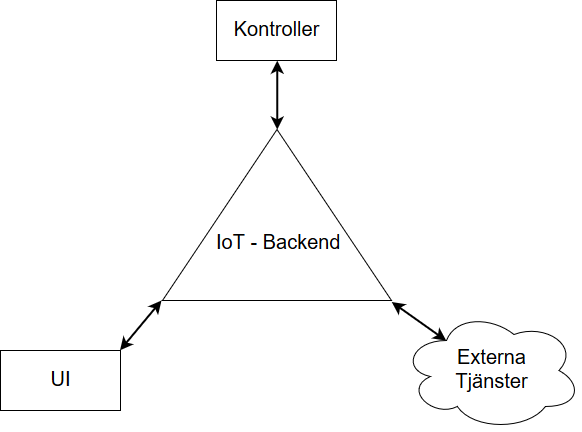
\includegraphics[scale=0.4]{backend}
		\caption{Kommunikation mellan Cybercoms IoT-backend och komponenterna i systemet}
		\label{fig:backend}
	\end{figure}
	
	
	\subsection{Beroenden av andra system}
	Produkten är beroende av Cybercoms IoT-backend då all kommunikation måste gå genom denna. Produkten är även beroende av en enhet som har tillgång till version 64 av Google Chrome. Produkten kräver även en enhet som kan köra UI-delen av systemet.

\pagebreak
\section{Krav}
	Detta avsnitt listar alla krav som sätts på produkten. Krav med prioritet 1 förväntas vara avklarade vid projektetsslut. Krav med prioritet 2 ska arbetas mot då alla krav med prioritet 1 är avklarade.
	\subsection{Funktionella Krav}
	Detta avsnitt listar de funktionella kraven på produkten.	
	
	\begin{tabular}{| p{2cm} | p{8cm} | p{2cm}|}
		\hline
		
		\textbf{Krav nr.} & \textbf{Beskrivning} &\textbf{Prioritet} \\ \hline
		Krav 1 & En mobil eller surfplatta ska användas som spelkontroll för spelet. & 1 \\ \hline
		Krav 2 & UI-applikationen ska stödja ett minimum av två spelare & 1 \\ \hline
		Krav 3 & Kontrollapplikationen ska ha ett grafiskt gränssnitt & 1 \\ \hline
		Krav 4 & UI-applikationen ska kunna köras på en enhet som har Google Chrome & 1 \\ \hline
		Krav 5 & Kontrollapplikationen ska kunna köras på en enhet som har Google Chrome & 1 \\ \hline
		Krav 6 & UI-applikationen ska endast kommunicera med \newline kontrollapplikation via  Cybercoms IoT-backend & 1 \\ \hline
		Krav 7 & UI-applikationen ska stödja version 64 av Google Chrome & 1 \\ \hline
		Krav 8 & Kontrollapplikationen ska stödja version 64 av Google Chrome & 1 \\ \hline
		Krav 9 & En användare ska kunna gå in i en spelinstans & 1 \\ \hline
		Krav 10 & UI-applikationen ska stödja hotjoinfunktionalitet & 1 \\ \hline
		Krav 11 & Flera instanser av spelet ska kunna köras samtidigt & 1 \\ \hline
		Krav 12 & En spelinstans spelare ska kunna rösta på vilket spel som ska spelas & 1 \\ \hline
		Krav 13 & UI-applikationen ska kunna starta en spelinstans & 1 \\ \hline
		Krav 14 & UI-applikationen ska kunna avsluta en spelinstans & 1 \\ \hline
		Krav 15 & Kontrollapplikationen ska kommunicera med Cybercoms IoT-backend & 1 \\ \hline
		Krav 16 & UI-applikationen ska kommunicera med Cybercoms IoT-backend & 1\\ \hline
		Krav 17 & En unik slumpmässig identifikationskod ska kunna genereras för en spelinstans & 1 \\ \hline
		Krav 18 & UI-Applikationen ska ha en knapp för att avsluta spelet & 1 \\ \hline
		Krav 19 & UI-applikationen ska kunna välja sin egna ID-kod för spelinstansen den kör & 2 \\ \hline
		Krav 20 & Kontrollapplikationen ska stödja styrning med tagentbord och mus & 2 \\ \hline
		Krav 21 & UI-applikationen ska visa en unik kod för sin spelinstans & 2 \\ \hline
		Krav 22 & Kontrollapplikationen ska kunna ansluta sig till en spelinstans genom att ange en identifikationskod & 2 \\ \hline
		
		
		
	\end{tabular}
	
	\subsection{Designkrav}
	Detta avsnitt listar kraven på utvecklingsprocessen
	
	\begin{tabular}{| p{2cm} | p{8cm} | p{2cm}|}
		\hline
		\textbf{Krav nr.} & \textbf{Beskrivning} & \textbf{Prioritet} \\ \hline
		
		Krav 22 & UI-applikationen ska skrivas i Javascript ES2015+ & 1 \\ \hline
		Krav 23 & Kontrollapplikationen ska skrivas i Javascript ES2015+ & 1 \\ \hline
		Krav 24 & UI-applikationen ska utvecklas som en PWA & 1 \\ \hline
		Krav 25 & Kontrollapplikationen ska utvecklas som en PWA & 1 \\ \hline
		Krav 26 & All kod som skrivs ska följa en dokumentationsstandard & 1 \\ \hline
		Krav 27 & UI-applikationen ska licensieras under MITs open source licens & 1 \\ \hline
		Krav 28 & Kontrollapplikationen ska licensieras under MITs open source licens & 1 \\ \hline
	\end{tabular}

	\subsection{Kvalitetskrav}
	Detta avsnitt listar krav på kvalitén hos den slutgilitga produkten.
	
		\begin{tabular}{|p{2cm}|p{8cm}|p{2cm}|}
		\hline
		\textbf{Krav nr.} & \textbf{Beskrivning} & \textbf{Prioritet} \\ \hline
		Krav 29 & UI-applikationen ska kunna köras i 4 timmar utan avbrott & 1 \\ \hline
		Krav 30 & Arkitekturen för systemet ska vara designat så att det är möjligt att vidareutveckla projektet & 1 \\ \hline
		Krav 31 & Tiden att ansluta sig till en spelsession får inte överskrida 10 sekunder under standard nätverksförhållanden & 1 \\ \hline
		Krav 32 & & \\ \hline
		
	\end{tabular}
	
\pagebreak

\printbibliography
\addcontentsline{toc}{section}{\refname}


\end{document}